% MARK: Preamble
\documentclass{thesis}

\usepackage{geometry}
\geometry{a4paper, margin=25mm}

\usepackage[utf8]{inputenc}
\usepackage[T1]{fontenc}
% Suppress scsl font not found error
\usepackage{silence}
\WarningFilter{latexfont}{Font shape `T1/cmr/m/scit' undefined}
\WarningFilter{latexfont}{Font shape `T1/cmr/m/scsl' undefined}

% Set paragraph seperation and indentation
\usepackage[%
    skip=1.0\baselineskip plus2pt,
    indent=20pt
]{parskip}
% Remove lineskip in itemize environment
\usepackage{enumitem}
\setlist[itemize]{nosep}
% Shorthand for blank line after a paragraph
% \newcommand{\prgph}%{}%{\vspace{\baselineskip}}

% Set the styling of captions
\usepackage[%
    hypcap=true,
    font=scriptsize,
    labelfont=bf,
    figurename=Figure,
    tablename=Table,
]{caption}
\usepackage{subcaption}

% MARK: Math packages
% Add: \degree and \micro,etc.
\usepackage{textcomp, gensymb}
% To get matrixes
% \usepackage{amsmath}
% Add additional math support, eg.: \lesssim
\usepackage{amssymb}
\usepackage{comment}
% \usepackage{mathtools}
\usepackage{siunitx}
% Provide sfrac command: $\sfrac{a}{b}$ -> a/b
% \usepackage{xfrac}

% MARK: Graphics packages
\usepackage{svg}
% Convert eps figures to pdf
% \usepackage{epstopdf}
% Allow custom in-text plots
\usepackage{pgfplots}
\pgfplotsset{compat=1.15}
% Include pdf documents in latex. Eg. for publications included in the appendix
% \usepackage{pdfpages}
% Allows you to work with graphics 
\usepackage{graphicx}
\graphicspath{%
    {chapter_0/figures/}%
    {chapter_1/figures/}%
    {chapter_2/figures/}%
    {chapter_3/figures/}%
    {chapter_4/figures/}%
    {chapter_5/figures/}%
    {chapter_6/figures/}%
}
% Add support for floats. I.E. floating
% \usepackage{float}
% programmatic-like interface to create highly customizable subfloats/subfigures
% \usepackage[farskip=0pt]{subfig}
% Allow figure text wrapping
% \usepackage{wrapfig}
% Allow rotation of tables
% \usepackage{rotating}
% Enhanced table setup
% \usepackage{ctable}
% Create tables that may continue to the next page
% \usepackage{longtable}

% MARK: Other packages
% Add support to split a table cell into multiple rows
\usepackage{multirow}
% Format tabular environments. Used by math and table packages
\usepackage{array}
% Allow strikethrough, eg.: \sout{example strikethrough text}
\usepackage{ulem}

% Section depth, e.g.: \S 1.1.1.1
% \setcounter{secnumdepth}{5}
% MARK: Custom hyperref
\usepackage{myhyperref}

% Control footnote layouts
% \usepackage[bottom, hang, flushmargin]{footmisc}
% Upright greek letters
% \usepackage{upgreek}
% 'robusify' the \subref command so it doesn't break on a whim
% \robustify{\subref}

% MARK: List 'include' files
\includeonly{%
    chapter_0/Abstract,
    chapter_0/Acknowledgements,
    chapter_0/Appendix_reduction,
    chapter_0/Appendix_code,
    chapter_1/Introduction,
    chapter_2/SALT_RSS_pipeline,
    chapter_3/Developed_tools,
    chapter_4/Testing_Application,
    chapter_5/Conclusions,
}

% Allow directory `tree' structures
\usepackage{dirtree}
% Allow relative font resizing.
\usepackage{relsize}

% MARK: Custom listings
\usepackage{mylistings}
% \usepackage[path=G:/STOPS/]{mylistings}

% https://www.overleaf.com/learn/latex/Using_colours_in_LaTeX &
% https://www.overleaf.com/learn/latex/Environments
% Allow text coloring
\usepackage{xcolor}

% MARK: Custom commands
\newcommand\todo[1]{{\noindent}\textcolor{red}{\textbf{TODO: #1}}}
% Hide TODO's
% \renewcommand\todo[1]{}
\newcommand{\Chapter}[2]{\chapter[#1]{#1:\\ \smallskip {\smaller[1] #2}}}

\newcommand{\angstrom}{\AA}
\newcommand{\arcmin}{\hbox{$^\prime$} }
\newcommand{\arcsec}{\hbox{$^{\prime\prime}$} }
\newcommand{\avg}[1]{\left< #1 \right> }
\newcommand{\degr}{\hbox{$^\circ$}}
\newcommand{\matr}[1]{\mathbf{#1}}

% Use numeric counting for footnotes
\renewcommand{\thefootnote}{\arabic{footnote}}

\newcommand{\super}[1]{\textsuperscript{#1}}
\newcommand{\rmn}[1]{{\mathrm{#1}}}

% \renewcommand{\arraystretch}{0.8}
% \renewcommand{\floatpagefraction}{.9}

% https://www.overleaf.com/learn/latex/Page_numbering
% Page numbering alteration
% \pagenumbering{Roman}

% MARK: Custom glossary
\usepackage{myglossary}

% Set the bibliography references
\usepackage[%
    round,
    colon,
    authoryear,
    sort&compress
]{natbib}
% Add bibliography to ToC
\usepackage[nottoc]{tocbibind}
% Set NASA ADS journal abbrevation macros
\usepackage{journal_macros}

% Fix Bibliography Underfull \hbox (badness 10000)
\usepackage{etoolbox}
\apptocmd{\sloppy}{\hbadness 10000\relax}{}{}

% Remnants from Hanno commands
\newcolumntype{P}[1]{>{\centering\arraybackslash}p{#1}}
% \setabbreviationstyle[longonly]{long}
% \setabbreviationstyle[shortonly]{short}
% \newabbreviation[category=longonly]{FSRQ}{FSRQ}{Flat Spectrum Radio Quasar}
% \newabbreviation[description={Interstellar Magnetic Fields}]{ISMF}{ISMF}{Interstellar Magnetic Fields}
% \newabbreviation[category=shortonly]{GRB}{GRB}{Gamma-ray Burst}

% MARK: 'thesis.cls' constants
\title{%
    \textbf{%
        Supplementary wavelength calibration methods for SALT/RSS spectropolarimetric observations
    }
}
\author{Justin Cooper}
\Cdegree{}% B.Sc. (Hons)}
\Sdegree{Magister Scienti\ae}
\university{University of the Free State}
\faculty{Faculty of Natural and Agricultural Sciences}
\department{Department of Physics}
\country{South Africa}
\degreedate{Date of submission: \today}
\supervisor{Prof. B. van Soelen}

% MARK: Main document
\begin{document}
% MARK: Front matter
\frontmatter
\maketitle
\clearpage

% MARK: Abstract
\begin{abstract}
    % Quick introduction
    % In one or two sentences give the goal of the thesis
    % Summarize the main findings of our results and how that is useful. State what we have done like you have done in Conclusions but only shorter

    \todo{
        \begin{itemize}
            \item Flow from use of SALT and pipeline and basics of its science implementations into why a more streamlined wavelength calibration is an improvement.
            \item Give summary of results.
            \item $<600$ words without going too in-depth into anything specific.
            \item Brian's comment: Abstract should summarize paper. Include results, conclusions, etc.
        \end{itemize}
    }

    % MARK: Keywords
    % TODO: Update myhyperref.sty with any additional keywords
    \textbf{Keywords:}
    \mykeywords
    %Polarization: optical,
    %galaxies: AGN,
    %Blazars,
    \todo{
        Pipeline development and data reduction keywords → look up the astronomy journal keywords ($\sim 10$ keywords)
    }
\end{abstract}

% https://jcap.sissa.it/jcap/help/helpLoader.jsp?pgType=kwList
% https://journals.aas.org/keywords-2013/
% https://academic.oup.com/DocumentLibrary/mnras/keywords.pdf
% https://www.aanda.org/for-authors/author-information/paper-organization
% https://www.raa-journal.org/sub/author/keywords/
% https://www.aip.de/en/astronomical-notes/instructions/keywords/

% MARK: HEASA 2021
% Blazars represent a subset of AGN with relativistic jets, where the direction of the jet lies very close to our line of sight. The highly Doppler boosted emission from the blazar's jet results in high apparent luminosities, and blazars display variability on periods from less than one day up to years. At optical wavelengths, the observed emission of the blazar is a superposition of the polarized non-thermal synchrotron emission, arising from the jet, and the non-polarized thermal emission, arising from the accretion disc, broad line region, torus and host galaxy.

% Polarimetry observations can serve as an important tool for diagnosing the emission from blazars. The RSS spectrograph, on SALT, can operate in spectropolarimetry mode and is currently being used to undertake spectropolarimetric observations of transient blazar sources.

% We present additional tools developed to work in conjunction with the current SALT spectropolarimetry reduction pipeline, {\sc polsalt}, that aims to streamline the reduction of the SALT polarization data, including the testing of the wavelength calibration of the individual O and E beams. This was applied to observations of 3C 279 during 2017.

% MARK: HEASA 2022
% Blazars are active galactic nuclei (AGN) with jets aligned very closely to our line of sight. The optical emission of blazars is often dominated by the polarized, non-thermal emission arising in the jets, with an underlying non-polarized, thermal emission component arising from the host galaxy, dusty torus, and accretion disk components.

% Coupled with multi-wavelength observations, optical spectropolarimetry of blazars during both flaring and quiescent states can be used to disentangle the polarized and non-polarized components in their spectral energy distributions, providing better constraints for the non-thermal particle distribution. To this end, spectropolarimetry of blazars during different states of activity was taken with the Southern African Large Telescope (SALT) using the Robert Stobie Spectrograph (RSS). For RSS spectropolarimetry, reductions are performed using the \textsc{polsalt} pipeline. In order to streamline the spectropolarimetric reductions, we have implemented supplementary interactive tools which provides additional wavelength calibration to improve the accuracy of the wavelength calibration for the O \& E beam.

% Here we present a brief overview of the tools and the results for Hiltner~652, a spectropolarimetric standard, as well as results for the blazars 3C~279. The reduced, $P_{Q}$ and $P_{U}$, Stokes parameters of Hiltner~652 show no major deviation from previously published results which reassures us that there is no interference introduced into the Stokes parameter calculations when wavelength calibrations are handled by our supplementary tools. The $\sim6000 - 9000$ Å range of 3C~279 shows a notable dip in the normalized spectrum during a period of flaring when compared to epochs of enhanced activity. The degree of polarization for 3C~279 of $13.2 \%$, $9.5 \%$, and $21.2 \%$ for the epochs 2017 March 28, 2017 March 31, and 2017 May 17, respectively, remains fairly constant across the observed wavelength ranges while still varying with the blazars' state of quiescence or flaring.

% MARK: Old Proposed Abstract
% Active Galactic Nuclei present the most energetic sources in the universe and are powered by the accretion of material onto a central supermassive black hole. These sources can show large relativistic jets which produce non-thermal radiation from radio to gamma-ray energies. Blazars, which are subdivided into Flat Spectrum Radio Quasars (FSRQs) and BL Lac objects, represent a subset of AGN where the direction of this jet lies very close to our line of sight. The highly Doppler boosted emission from the jet, results in high apparent luminosities and blazars display variability on periods from less than one day up to years. The Spectral Energy Distribution (SED) of blazars shows two clear components: a low energy component which is produced through electron synchrotron radiation (radio to UV/X-ray) and a high energy component which is produced through either inverse Compton scattering of soft target photons or hadronic processes (e.g. π 0 decay, proton synchrotron). In some of these sources the high energy component extends to observable Very High Energy (VHE) gamma-rays.

% The blazar sub-class FSRQs have accretion discs (as shown by the strong emission lines in the optical spectra) and this means observations at optical wavelengths include a superposition of thermal emission, primarily from the accretion disc, and non-thermal radiation from synchrotron radiation originating from the jet. One of the difficulties in modelling FSRQs is to disentangle the contribution of the different components. One method, which is being employed is to look at the degree of linear polarization, since this arises from the synchrotron emission, and to simultaneously model both the flux and the degree of polarization.

% As part of the SALT Large Science Proposal Observing the Transient Universe, the AGN working group is using the RSS spectrograph on the Southern African Large Telescope (SALT) to observe blazars during gamma-ray flaring/non-flaring states in spectropolarimetry mode, with quasi-simultaneous photometric optical observations undertaken with the LCO and/or Master network. This allows the degree of polarization to be directly measured (Fig. 1) and allows us to self-consistently model the low energy component of blazars, differentiating the underlying components (see Fig. 2).

% The aim of the proposed Masters project will be to further develop the methodology to undertake observations of flaring blazars, take a leading role in triggering observations with SALT and the other telescope networks, the reduction and analysis of the observations, and develop the necessary pipelines to “stream-line” the observations. These observations will then serve as the input for modelling the emission, in collaboration with other members of the AGN working group, primarily Markus Böttcher and Hester Schutte.

% A working knowledge of IRAF and Python will be an important skill required for this project.

% MARK: CHATGPT Abstract

% The Southern African Large Telescope (SALT) Robert Stobie Spectrograph (RSS) provides valuable data through spectropolarimetric observations, essential for understanding astrophysical objects and processes, such as active galactic nuclei. However, the current wavelength calibration methods, which are pivotal for accurate data analysis, are complex and time-consuming. This thesis presents supplementary wavelength calibration tools aimed at improving the efficiency and accuracy of data reductions for spectropolarimetry using SALT/RSS. The development of the Supplementary Tools for polsalt Spectropolarimetry (STOPS) addresses limitations in the existing polsalt software, including enhancements in splitting, joining, skyline subtraction, and cross-correlation routines. The implementation of these tools offers a more streamlined calibration process, reducing observational errors and improving data quality. The results demonstrate the enhanced performance of STOPS in reducing spectropolarimetric data and its potential application in future observations. The tools are validated through a series of test cases and real-world data, highlighting their effectiveness in improving the reliability and accuracy of SALT/RSS observations.
% MARK: Dedication
\begin{dedication} \noindent

    \vspace{\stretch{1}}

    In loving memory of my grandpa and oupa,

    \vspace{\baselineskip}

    \textbf{Boyd McGowan Fichardt Cooper} \\
    $1942 - 2021$

    \vspace{\baselineskip}

    \textbf{Jacobus Pieter (Koos) van der Merwe} \\
    $1947 - 2024$

    \vspace{\stretch{2}}

\end{dedication}

% MARK: Acknowledgements
\begin{acknowledgements}
    I hereby acknowledge and express my sincere gratitude to the following parties for their valuable contributions:
    \begin{itemize}
        \item To my supervisor, Prof. Brain van Soelen: Dear `sir', thank you for your guidance and patience.
        \item To my parents, Afrikaans and English, near and far, and those who love me as one of their own, you are the foundation upon which I am built.
        \item To my friends, thank you for always offering (sometimes poor) words of wisdom and encouragement.
        \item To the personnel at the Department of Physics (UFS)
        % \item The team at \gls{SAAO}/\gls{SALT}, specifically David Buckley and Danièl Groenewald for their time and expertise.
        % All/some [choose which is appropriate] of the observations reported in this paper were obtained with the Southern African Large Telescope (SALT) under program(s) [insert Proposal Code(s)].
    \end{itemize}
\end{acknowledgements}

\tableofcontents

\printglossary[type=\acronymtype, style=super, title={List of Acronyms and Symbols}]

% MARK: Main matter
\mainmatter
\chapter{Introduction}
% 1 Section summary of research. More complete abstract without results.
\todo{
    Very short intro to Spectroscopy, Polarisation, and Spectropolarisation and their Importance in astronomy
}

\todo{
    Problem Statement, \textbf{VERY IMPORTANT}, roughly a sentence but problem thoroughly fleshed out.
}

\todo{
    Focus on AGN implications and implementations such as the types of objects and a short history for each type of object, Blazar focus with specification on BL Lacs and FSRQs, the Unified Model, \sout{The Blazar sequence}
}

\todo{
    Brian's comment: Highlight importance of polarimetry for understanding emission and how that plays a role in AGN.
}

\todo{
    Basics of modelling (Different energy/wavelength ranges used and what the models tell us about emission processes/structure) so that Hester's results can be noted for applications of the pipeline.
}

\todo{
    General layout of Dissertation
}

\chapter{Spectropolarimetry and the SALT RSS}

This chapter gives a brief overview of the basics of spectropolarimetry and how it functions based off of the principles of both spectroscopy and polarimetry. Further, it is discussed how these techniques are practically implemented for \gls{SALT}, and more specifically the \gls{RSS}, and how the spectropolarimetric reduction process is completed.

\section{Spectroscopy}

% History
Spectroscopy originated in its most basic form with Newton's examinations of sunlight through a prism \citep{opticks} but came to prominence as a field of scientific study with Wollaston's improvements to the optics elements \citep{WollPrism}, Fraunhofer's use of a diffraction grating instead of a prism as a dispersion element \citep{FraunGrating}, and Bunsen and Kirchoff's classifications of spectral features to their respective chemical elements \citep{KirBunSpec}.
\prgph

\begin{figure}[t]
    \centering
    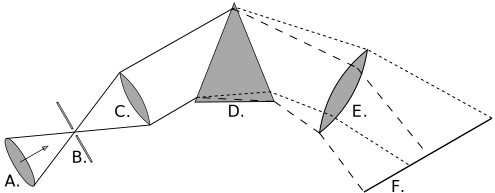
\includegraphics[width = 0.9\textwidth]{figures/2_spectrometer.pdf}
    \caption{Layout depicting the path light collected by a telescope would travel through a simple spectrometer.}
    \label{fig:spectrometer}
\end{figure}

% How it works
The simplest spectrometer schematic as shown in Figure \ref{fig:spectrometer} consists of incident light collected from the telescope's optics, labeled A, being focused onto a slit, labeled B, and passed through a collimator, labeled C. The collimator collimates the light allowing a dispersion element (such as a diffraction grating or prism), labeled D, to disperse the light into its constituent wavelengths. The resultant spectrum is focused by a focusing lens, labeled E, onto a focal plane, labeled F. Viewing optics are situated at the focal plane in the case of a spectroscope and a detector is situated at the focal plane in the case of a spectrograph.
\prgph

% Telescope optics
The telescope optics refers simply to all the components of a telescope necessary to acquire a focal point where the spectrometer, components labeled B - F, is situated. The focal point in most traditional telescope designs is fixed relative to the telescope and so the spectrometer may be mounted at that point. In cases where the telescope is designed to have a moving focal point relative to the telescope \cite[see][]{Arecibo, HET, SALT_design}, the spectrometer must also move along the telescope's focal path.
\prgph
\prgph

% SLIT
The slits function is to control the amount of incident light entering a spectrometer and, along with the exposure time of the detector, prevents over-exposures of bright sources on highly sensitive detectors \citep{TonkPracAmSpec}. If a source is spatially resolvable, or larger than the seeing conditions, the slit further acts to spatially limit the source to increase the spectral resolution, resulting in sharper features in the resultant spectrum.
\prgph

Without a slit the spectral resolution would be determined by the projected width of the source on the detector, or the seeing if the source was a star-like point source. Increasing the spectral resolution comes with the trade-off of decreasing the light collected from the source and thus acquiring a less intense resultant spectrum. Multiple spectra may be acquired simultaneously when the slit is positioned such that collinear sources lie along the slit.
%Spectroscopy done with no slit is commonly referred to as objective spectroscopy and, as the name suggests, the prism is situated just before the telescopes objective, the primary element of the telescope that focuses the collected light to the primary focus.
\prgph

% COLLIMATOR
The collimating lens functions to collimate the focused light from the telescope, ensuring that all light rays run parallel before reaching the dispersion element. Since the collimator accounts for the telescope's focus, the focal ratio of the collimator, $f_{1} / d_{1}$, should thus optimally match the focal ratio of the telescope, $f / D$, as seen in Equation \ref{eq:focal_ratio} to be most efficient and to not waste collecting area or material on too large a collimator.
% \prgph

\begin{equation}
	\frac{f}{D} = \frac{f_{1}}{d_{1}}
	\label{eq:focal_ratio}
\end{equation}

% From basic trigonometry and a small angle approximation, $\sin(\theta) \approx \theta$, Equation \ref{eq:small_angle} can be derived. From it, it can be seen that as the linear size, $D$, of most stellar objects is much smaller than the distance to those objects, $d$, and thus the incident light is already almost entirely collimated.

% \begin{equation}
% 	\theta (\arcsec) = 206265 \frac{D}{d}
% 	\label{eq:small_angle}
% \end{equation}

% DISPERSION ELEMENT
The dispersion element is the element that defines a spectrometer. As the name suggests, a dispersion element disperses the light incident on it into its constituent wavelengths and produces a spectrum. There are two types of dispersion elements, namely the prism and the diffraction grating, which operate on different principles, as discussed in Section \ref{subsec:dispersion}.
\prgph

% Focusing lens and FOCAL PLANE / Detector / Camera / CCD
% Can use \citep{CMOS_use} for CMOS use in general spectroscopy
%  - Spectroscopy and Spectrography
The focusing lens functions similarly to that of the telescope's optics but in this case focuses the dispersed light onto some receiver situated at the focal plane. As mentioned previously, an eye piece is fixed to the focal point for a spectroscope while a spectrograph employs a detector.
\prgph

The two most prevalent detector types in spectroscopy are the \gls{CCD} and \gls{CMOS} detectors. In astronomical spectroscopy however, sources are fainter and exposure times are much longer and so the \gls{CCD} detectors are by far the preferred detector as their output has a higher-quality and lower-noise when compared to \gls{CMOS} cameras under the same conditions \citep{CCDvsCMOS}.
\prgph

The \gls{CCD} is a detector composed of many thousands of pixels which can store a charge so long as a voltage is maintained across the pixels. Each pixel detects incoming photons using photo-sensitive capacitors through the photoelectric effect and converts the photons to a charge \citep{CCDastronomy}. There are also thermal agitation effects which introduce noise to the charge accumulated by a pixel, further discussed in Section \ref{subsec:calibration}. Once the exposure is finished the accumulated charge is read column by column, row by row, through an \gls{ADC}  which produces a two-dimensional array of `counts' with which information may be extracted from. Each \gls{CCD} image may be referred to by a name such as a bias, dark, flat field, or science image, which helps the observer differentiate the purpose of each image, also further discussed in Section \ref{subsec:calibration}.

\subsection{Dispersion Elements} \label{subsec:dispersion}
% https://spectroscopy.wordpress.com/2020/05/12/basics-on-prisms-and-diffraction-gratings-part-1/

Light can be broken up into its constituent wavelengths through two different physical phenomena, namely dispersion and diffraction, which dispersive elements use to create spectra. Dispersive prisms and diffractive gratings each have their strengths and weaknesses and a wide spectrum of instruments exist implementing both, or either, concepts. Regardless of the specific element, dispersive elements all have a resolving power, $R$, and an angular dispersion. Generally, while the angular dispersion is a more involved process to determine, the resolving power of a spectrograph can be measured as:
% \prgph

\begin{equation}
	R = \frac{\lambda}{FWHM}
    \label{eq:resolving_power}
\end{equation}

\noindent where $\lambda$ is the wavelength of an incident monochromatic beam and $FWHM$ refers to the width of the feature on the detector at half of its maximum intensity.
\prgph

%   - Prism
\begin{figure}[t]
    \centering
    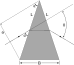
\includegraphics[width = 7cm]{figures/2_prism_diagram.pdf}
    \caption{Geometry of a prism refracting an incident monochromatic beam at a minimum deviation angle.}
    \label{fig:prism_diagram}
\end{figure}

The prism operates on the principle that the refractive index of light, $n$, varies as a function of its wavelength, $\lambda$. Prisms were the only dispersive elements available for early spectroscopic studies, but they were not without flaw.
% \prgph

\begin{equation}
	\frac{\partial \theta}{\partial \lambda} = \frac{B}{a}\frac{dn}{d\lambda}% \propto -\lambda^{-3}
    \label{eq:prism_angular_dispersion}
\end{equation}

The angular dispersion of a prism can be represented by Equation \ref{eq:prism_angular_dispersion} where the variables relate to Figure \ref{fig:prism_diagram} such that $\theta$ is the angle at which the refracted light differs from the incident light, $\lambda$ is the wavelength of the incident light, $B$ is the longest distance the beam would travel through the prism, and $a = L \sin(\alpha)$ is the cross-section of the incident beam where $L$ is the length of the transmissive surfaces and $\alpha$ is the incident angle of light to the prism surface. The refractive index of a material as a function of its wavelength, $n(\lambda)$, has several equations. Cauchy's equation, as given in Equation \ref{eq:Cauchy}, is a much simpler approximation of the refractive index that remains very accurate at visible wavelengths.
% \prgph

\begin{equation}
	n(\lambda) = A_{C} + \frac{B_{C}}{\lambda^{2}} + \frac{C_{C}}{\lambda^{4}} + \dots
    \label{eq:Cauchy}
\end{equation}

Equation \ref{eq:Cauchy}'s $A_{C}, B_{C}, C_{C}, \dots$ variables are called the Cauchy coefficients and have known values dependent on the material. Taking only the first term of the derivative of the Cauchy equation allows us to approximate the angular dispersion of a prism.

\begin{equation}
	\frac{\partial \theta}{\partial \lambda} = -\frac{B}{a}\frac{2B_{C}}{\lambda^{3}} \propto -\lambda^{-3}
    \label{eq:prism_angular_dispersion_approx}
\end{equation}

Equation \ref{eq:prism_angular_dispersion_approx} shows that the angular dispersion of a prism is wavelength dependent and furthermore that longer wavelengths are dispersed less than shorter wavelengths \citep{BirneyObsAstro, Hecht_optics}. The dependence of the angular dispersion, $d\theta/d\lambda$, on the wavelength, $\lambda$, is crucial for the formation of a spectrum but this cubic, non-linear, relation results in a non-linear spectrum. Since prisms rely on the refractive index of the material they are made of they have low angular dispersions.
\prgph

Multiple prisms can be used to increase the angular dispersion but as the dispersion is non-linear it becomes increasingly more difficult to calibrate. The more material and material boundaries the light must pass through the more its intensity decreases due to attenuation effects and Fresnel losses. Even so, the transmittance of modern prisms for their selected wavelength range is generally very high due to improved manufacturing methods as well as improved transmitting materials.
\prgph

%   - Diffraction grating
\begin{figure}[t]
    \centering
    
\includegraphics[width = 9cm]{figures/2_grating_diagram.pdf}
    \caption{Geometry of a reflective blazed grating refracting\\an incident monochromatic beam}
    \label{fig:grating_diagram}
\end{figure}

The diffraction grating operates on the principle that when light interacts with a grating where the groove size is comparable to the light's wavelength, the light is dispersed as a function of its wavelength through constructive and destructive interference. This interference results in multiple diffracted beams $m$, called orders, either side of a central reflected, or transmitted, beam such that $m \in Z$, where $m = 0$ is the non-dispersed, or reflected, beam.
% \prgph

\begin{equation}
	m\lambda = \sigma (\sin(\alpha) \pm \sin(\beta))
    \label{eq:grating_equation}
\end{equation}

% Link eq and fig
Equation \ref{eq:grating_equation} is referred to as the grating equation and its variables relate to Figure \ref{fig:grating_diagram} such that $m$ is the order of the diffracted beam being measured, $\lambda$ is the wavelength of the incident light, $\sigma$ is the groove spacing, $\alpha$ is the angle of incident light relative to the grating normal, and $\beta$ is the angle of diffraction relative to the grating normal. It is important to note that the sign of $\alpha$ and $\beta$ depend on whether the grating is reflective or transmissive. In the case of a reflective grating, such as in Figure \ref{fig:grating_diagram}, the signs of $\alpha$ and $\beta$ are the same relative to the grating normal, I.E. $\lambda = \sigma (\sin(\alpha) + \sin(\beta))$ for $m = 1$. In the case of a transmissive grating, the signs of $\alpha$ and $\beta$ are the opposite relative to the grating normal, I.E. $\lambda = \sigma (\sin(\alpha) - \sin(\beta))$ for $m = 1$.
\prgph

% Free Spectral range and Blazing
Equation \ref{eq:grating_equation} also describes how multiple wavelengths can share an angle of refraction when $m\lambda_{m} = (m + 1)\lambda_{m + 1}$. The regions of an order that do not overlap with another order are called the free spectral range. To account for the overlaps and increase the free spectral range an order-blocking filter may be used, and the diffraction grating may be blazed by an angle, $\theta$, such as in Figure \ref{fig:grating_diagram}. Blazing refers to the fact that the grooves on the surface of the grating are not symmetrical. The asymmetry of the grooves diffract the incident beam such that most of the incident beam's intensity is focused to a single order for a designated `blazed' wavelength, $\lambda_{b}$.
% \prgph

\begin{equation}
	m\lambda_{b} = 2\sigma\sin(\theta)\cos(\alpha - \theta)
    \label{eq:blaze_wavelength}
\end{equation}

\noindent where

\begin{equation}
    2\theta = \alpha + \beta
\end{equation}

% Angular dispersion
Taking the derivative of Equation \ref{eq:grating_equation} with respect to $\lambda$ and keeping $\alpha$ constant allows us to determine the angular dispersion of a diffraction grating.

\begin{equation}
    \frac{\partial \beta}{\partial \lambda} = \frac{m}{\sigma \cos(\beta)}
    \label{eq:grating_angular_dispersion}
\end{equation}

\noindent Substituting $m / \sigma$ with the grating equation gives

\begin{equation}
    \frac{\partial \beta}{\partial \lambda} = \frac{\sin(\alpha) + \sin(\beta)}{\lambda \cos(\beta)} \propto \lambda^{-1}
    \label{eq:grating_angular_dispersion_approx}
\end{equation}

Similarly to the dispersion of a prism, Equation \ref{eq:grating_angular_dispersion_approx} shows that the dispersion of a grating is wavelength dependent, but this dependence is only inversely proportional and thus more uniform across a wavelength range than that of a prism. Furthermore, shorter wavelengths are refracted less than longer wavelengths since there is no negative relation between the angular dispersion and the wavelength \citep{BirneyObsAstro, Hecht_optics}.
\prgph

% Grism and immersed grating
As mentioned before, multiple subgroups exist for both dispersive prisms and diffractive gratings. For prisms, along with the single and multiple prism setups mentioned above, there also exist grisms and immersed gratings. A grism (Grating Prism) refers to a transmissive grating etched onto one of the transmissive faces of a prism and allows a single camera to capture both spectroscopic and photometric images without needing to be moved, with and without the grism in the path of the beam of light, respectively. An immersed grating refers to a grism modified such that the transmissive grating is coated with reflective material. The primary source of dispersion for both grisms and immersive gratings is the grating and any aberration effects from the prism are negligible in comparison.
\prgph

\begin{figure}[t]
    \centering
    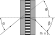
\includegraphics[width = 10cm]{figures/2_vph_grating.pdf}
    \caption{Geometry of a \gls{VPH} grating for an incident monochromatic beam of light.}
    \label{fig:vph_grating}
\end{figure}

% Echelle and VPH grating
% https://www.astro.ljmu.ac.uk/~ikb/vph.html
For gratings, along with transmissive and reflective gratings there also exist \gls{VPH} gratings. A \gls{VPH} grating consists of a photoresist, which is a light-sensitive material, sandwiched between two glass substrates. Diffraction is possible since the photoresist's refractive index varies near-sinusoidally perpendicularly to the gratings lines. This allows for sharper diffraction orders and low stray light scattering as compared to more traditional gratings but since blazing is not possible the efficiency is decreased. An echelle grating refers to two gratings set up such that the dispersed light from one is further diffracted by a second and allows for comparatively higher spectral resolutions when compared to more traditional grating setups. The gratings used as part of the echelle grating may be any type of dispersion element, but gratings are traditionally preferred due to the linearity of their resultant spectrum.
\prgph

\subsection{Detector and Spectroscopic Calibrations}\label{subsec:calibration}

Acquiring a spectrum from observations is more involved than simply reading out the data recorded on the \gls{CCD}. A raw science image, which is the raw counts of the observed source read from the \gls{CCD} with no calibrations applied, has on it a combination of useful science data as well as noise. The noise is a combination of random noise introduced through statistical processes and systematic noise introduced through the instrumentation and the observation conditions the source was observed under. This noise causes an uncertainty in the useful data and can be minimized, predominantly by calibrating for the systematic noise, but never fully removed \citep{CCDhandbook}.
\prgph

The dominant source of noise in a raw image is detector noise. \gls{CCD}'s are manufactured to have a small base charge in each pixel, called the `bias' current which allows the readout noise, a type of random noise, to better be sampled. There is also an unintentional additional charge which is linearly proportional to the exposure time and originates from thermal agitation of the \gls{CCD} material, called the `dark' current. The dark current can be minimized and possibly ignored if the \gls{CCD} is adequately cooled. These types of noise add to the charge held by a pixel and are thus considered additive.
\prgph

The \gls{CCD} is not a perfect detector and the efficiency of it and the optics of the telescope also contribute noise to the image. The efficiency of a \gls{CCD} is referred to as the Quantum Efficiency, and it is a measure of what percentage of light striking the detector is actually recorded and converted to a charge. The efficiency of the \gls{CCD} and telescope optics is also wavelength dependent and so the noise that results from them is more complex than that of additive noise. This type of noise is referred to as multiplicative noise.
\prgph

Each image taken by a \gls{CCD} will inherently have the additive types of noise in the image, and so bias and dark currents are the first types of noise to be accounted for by subtracting them from any subsequent images. Bias currents can be found by taking a bias image or by adding an overscan region to each image. A bias image is an image where the charges on the \gls{CCD} are reset and then immediately read off without exposing anything on the detector, effectively taking an image with zero exposure time. Alternatively, to save time during an observational run, overscan regions may be added to the images. An overscan region refers to adding a few cycles to the readout of each column of the \gls{CCD} such that the base current is read out and appended to each image.
\prgph

Dark currents can be found by taking an image with nothing exposed onto the detector for a certain exposure time. This resultant dark image can then be scaled to the science images exposure time since the dark current is linearly proportional to exposure time. When the detector is capable of being held at precise temperatures, dark images may be taken over multiple hours during the day to produce a high quality master dark image that may then be scaled and subtracted from all subsequent images.
\prgph

After the additive noise has been accounted for, the response from the pixels detecting the same incoming light are still not all the same due to the multiplicative noise which still needs to be accounted for. An image that has this noise accounted for is considered to be flat since all pixels share the same response to the incoming light. This noise can be measured by taking a `flat' image, or alternatively a flat-field, and multiple types of flats can be taken which all in essence image a uniformly illuminated region to determine the pixel-to-pixel response.
\prgph

Night sky flats are produced from science images where the images contain mostly sky. The science images are combined using the mode statistic which removes any celestial objects. This allows science images to be used for flat-fielding but at the cost of having a low \gls{SNR} because of the dim background sky. Dome flats are images taken of a flat surface inside the telescopes dome that has been uniformly and indirectly illuminated. These flats allow precise control of the light source and are also capable of being taken during the day. Finally, twilight flats are images taken of the twilight (or dawn) sky, when the Sun has just set, opposite the direction of the Sun at about $20\degr$ from zenith. Careful planning is required for twilight flats as the sky's brightness changes rapidly with the setting and rising of the Sun.
\prgph

A flat-field must be normalized before being used to correct any science images since it only acts to account for the pixel-to-pixel response and not for the additive errors. The normalized flat image, $F^{n}_{\lambda}(x,y)$ can be calculated as:

\begin{equation}
    F^{n}_{\lambda}(x,y) = \frac{F_{\lambda}(x,y) - B(x,y) - (\frac{t_{S}}{t_{D}})D(x,y)}{mode(F_{\lambda}(x,y) - B(x,y) - (\frac{t_{S}}{t_{D}})D(x,y))}
    \label{eq:norm_flat}
\end{equation}

\noindent where $F_{\lambda}(x,y)$ is the non-corrected flat image, $B(x,y)$ is the bias image, $D(x,y)$ is the dark image which is scaled by $t_{S}$ and $t_{D}$, the science image and dark image exposure times, respectively.
\prgph

The calibrated science image, $S^{*}_{\lambda}(x,y)$, which accounts for the bias and dark currents as well as the flat fielding can then be calculated as:

\begin{equation}
    S^{*}_{\lambda}(x,y) = \frac{S_{\lambda}(x,y) - B(x,y) - (\frac{t_{S}}{t_{D}})D(x,y)}{F^{n}_{\lambda}(x,y)}.
    \label{eq:science_cal}
\end{equation}

Multichannel \gls{CCD}'s are detectors that use either multiple \gls{CCD}'s or a \gls{CCD} with multiple output amplifiers which can be read out through multiple channels at the same time, increasing the detectors size while keeping the readout time constant. These \gls{CCD} setups need additional calibrations, specifically cross-talk corrections and mosaicking.
\prgph

Cross-talk noise refers to contamination that occurs during readout in one channel from another channel with a high signal and occurs because the signals can not be completely isolated from one another. Cross-talk corrections therefore account for this signal contamination between channels being read out at the same time \citep{CrossTalk}. Mosaicking is necessary for multichannel \gls{CCD}'s since the digitized signal read out from the detector has no reference of the physical location of the pixel it was detected at. Mosaicking therefore orients the data acquired from a multichannel detector correctly relatively to one another so that a single image is produced from the multiple channels read out from the detector.
\prgph

Finally, calibrations necessary for spectroscopy are limited to wavelength calibrations. Since the dispersion element breaks the incident light into its constituent wavelengths non-linearly, as discussed in Section \ref{subsec:dispersion}, the relation between the pixel on a detector and the wavelength of the light incident on it is unknown. Ideally, the spectrometer's optics would be modeled to produce a reliable pixel to wavelength calibration \citep[see E.g.][]{WavCalSpectraModel}, but this becomes increasingly more difficult for spectrometers with complex, non-sedentary, optical paths. Alternatively, a source with well-defined spectral features, with said features evenly populating the wavelength region of interest, such as in Figure \ref{fig:Ne_arc} may be observed. The observed frame is commonly referred to as an `arc' frame, after the arc lamps used to acquire the spectra, and should be observed alongside the science frames over the course of an observation run. It is important that the arc frame is observed at the same observing conditions and parameters as the science frames since the optical path will vary over the course of an observing run and for different observing parameters, invalidating previously acquired arc frames.
\prgph

\begin{figure}[t]
    \centering
    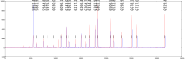
\includegraphics[width = 16cm]{figures/2_Ne_arc.pdf}
    \caption{Example of an arc spectrum for NeAr taken with \gls{SALT}'s \gls{RSS} using the PG1800 grating at a grating angle of $34.625$°, an articulation angle of $69.258$°, and covering a wavelength range of $\sim5600 - 6900$\angstrom. Plot adapted from \gls{SALT}'s published Longslit Line Atlases (as of 2023)\protect\footnotemark}
    \label{fig:Ne_arc}
\end{figure}
\footnotetext{\protect\href{http://pysalt.salt.ac.za/lineatlas/plot_line_neon.pdf}{NeAr plot} sourced from \protect\url{https://astronomers.salt.ac.za/data/salt-longslit-line-atlas/}}

The wavelength calibrations then consist of identifying a two-dimensional pixel to wavelength conversion function from the arc frame which may later be applied to calibrate the science frames. The two most common approximations for wavelength calibrations are the Chebyshev and Legendre polynomial approximations as found in Equations \ref{eq:chebyshev} and \ref{eq:legendre}, respectively. The Chebyshev polynomials are defined explicitly as:

\begin{equation}
    T_{n}(x) = \cos(n \cos^{-1}(x)),
    \label{eq:chebypolyexplicit}
\end{equation}

\noindent or recursively as:
\begin{equation}
    \begin{gathered}
        T_{0}(x) = 1 \\
        T_{1}(x) = x  \\
        T_{n}(x) = 2 x T_{n - 1}(x) - T_{n - 2}(x), \text{ for } n > 1
    \end{gathered}
    \label{eq:chebypoly}
\end{equation}

\noindent where $T$ is a Chebyshev polynomial\footnote{Denoted $T$ as a hold-over from the alternate spelling, `Tchebycheff'.} of degree $n$. Chebyshev polynomials are orthogonal when weighted by $1 / \sqrt{1 - x^{2}}$, meaning that the inner product of any two different polynomials, $T_{i}(x)$ and $T_{j}(x)$, over the range of $[-1, 1]$ is zero.

\begin{equation}
    \int_{-1}^{1} T_{i}(x) T_{j}(x) \frac{1}{\sqrt{1-x^{2}}} \,dx =
    \begin{cases}
        0,       & i \neq j\\
        \pi / 2, & i = j \neq 0\\
        \pi,     & i = j = 0
    \end{cases}
    \label{eq:chebyorth}
\end{equation}

A one or two-dimensional unknown calibration function may then be approximated by Chebyshev polynomials using:

\begin{equation}
    f(x) \approx \sum_{i = 0}^{N}  c_{i} T_{i}(u)
    \label{eq:chebyshev}
\end{equation}

\noindent or

\begin{equation}
    F(x, y) \approx \sum_{i = 0}^{N} \sum_{j = 0}^{M} c_{ij} T_{i}(u) T_{j}(v),
    \label{eq:chebyshev2D}
\end{equation}

\noindent respectively, where $N$ and $M$ are the desired $x$ and $y$ orders, $c_{ij}$ are the Chebyshev polynomial coefficients, and $u, v \in [-1, 1]$ are scaling factors to remap the variables $x, y \in [a, b]$ such that the orthogonality property of the Chebyshev polynomials holds true \citep{chebysurf, cheby2d}.

\begin{align}
    (u, v) &= \frac{2 (x, y) - a - b}{b - a} & (x, y) &= \frac{b - a}{2} (u, v) + \frac{a+b}{2}
    \label{eq:XtoUV}
\end{align}

% When the calibration function is known but the function cannot be evaluated, the coefficients, $c_{n}$, may be approximated by:

% \begin{equation}
%     c_{n} \approx \frac{2}{N} \sum_{k = 0}^{N - 1} f(x_{k}) T_{n}(x_{k})
%     \label{eq:chebycoeff}
% \end{equation}

% \noindent where:

% \noindent which returns the positions of the  x-intercepts.
% \prgph

The Chebyshev polynomials are more ideally suited for wavelength calibrations than standard polynomials since they are orthogonal and have minima and maxima located at $[-1, 1]$, as seen in Figure \ref{fig:chebyshev}. This means that the Chebyshev approximation is exact when $x = x_{n}$, where $x_{n}$ are the positions of the $n - 1$ x-intercepts of $T_{N}(x)$. This property greatly minimizes the error in the Chebyshev approximation, even at lower order approximations \citep{cheby}.

\begin{equation}
    x_{n} = \cos{\left(  \frac{\pi}{2} \frac{2 n + 1}{N} \right)}
\end{equation}

% \prgph

\begin{figure}[t]
    \centering
    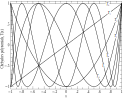
\includegraphics[width = 12cm]{figures/2_chebyshev.pdf}
    \caption{The first seven Chebyshev polynomials ($T_0$ through $T_{6}$) as defined by Equation \ref{eq:chebypoly} over the region $[-1, 1]$ for which they are orthogonal. Figure adapted from \citep{numerical_recipes} (2023)\protect\footnotemark}
    \label{fig:chebyshev}
\end{figure}
\footnotetext{Available digitally at \protect\href{http://numerical.recipes/book}{numerical.recipes}}

Similar to the Chebyshev polynomials, the Legendre polynomials may be defined explicitly as:

\begin{equation}
    P_{n}(x) = \frac{1}{2^{n} n!} \frac{d^{n}}{d x^{n}} (x^{2} - 1)^{n}
    \label{eq:legpolyexplicit}
\end{equation}

\noindent or recursively as:

\begin{equation}
    \begin{gathered}
        P_{0}(x) = 1 \\
        P_{1}(x) = x \\
        P_{n}(x) = \frac{2 n + 1}{n + 1} x P_{n - 1}(x) - \frac{n}{n + 1} P_{n - 2}(x), \text{ for } n > 1
    \end{gathered}
    \label{eq:legpoly}
\end{equation}

\noindent where P is a Legendre polynomial of degree n. Legendre polynomials are also orthogonal over the range $[-1, 1]$.
\prgph

\begin{equation}
    \int_{-1}^{1} P_{i}(x) P_{j}(x) \,dx =
    \begin{cases}
        0,                 & i \neq j\\
        \frac{2}{2 n + 1}, & i = j
    \end{cases}
    \label{eq:legorth}
\end{equation}

A one or two-dimensional unknown calibration function may then be approximated by Legendre polynomials using:

\begin{equation}
    f(x) \approx \sum_{n = 0}^{N} a_{n} P_{n}(u)
    \label{eq:legendre}
\end{equation}

\noindent or

\begin{equation}
    F(x, y) \approx \sum_{i = 0}^{N} \sum_{j = 0}^{M} a_{ij} P_{i}(u) P_{j}(v),
    \label{eq:Legendre2D}
\end{equation}

\begin{figure}[t]
    \centering
    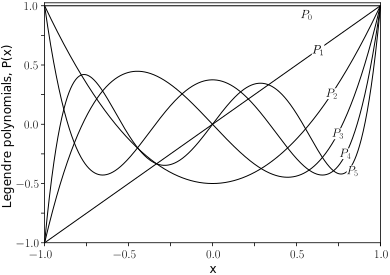
\includegraphics[width = 12cm]{figures/2_legendre.pdf}
    \caption{The first six Legendre polynomials ($P_0$ through $P_{5}$) as defined by Equation \ref{eq:legendre} over the region $[-1, 1]$ for which they are orthogonal. Figure adapted from Geek3, \protect\href{https://creativecommons.org/licenses/by-sa/3.0}{CC BY-SA 3.0}, via \protect\href{https://commons.wikimedia.org/wiki/File:Legendrepolynomials6.svg}{Wikimedia Commons} (2023)}
    \label{fig:legendre}
\end{figure}

\noindent respectively, where $N$ and $M$ are the desired $x$ and $y$ orders, $u$ and $v$ are the same mapping variable as in Equation \ref{eq:XtoUV}, and $a_{ij}$ are the Legendre polynomial coefficients. Legendre polynomials benefit from having the orthogonality condition with no weight necessary which makes their coefficients easier to compute but the error in a Legendre approximation of a function is greater than that of the error in a Chebyshev approximation for the same required order, $N$ (in one dimension) \citep{leg_cheb_relation}.
\prgph

Regardless of which set of polynomials is chosen, the polynomials are fit to the known (wavelength, pixel) pair using the least squares method. The resultant minimized function may then be used to convert the science frames from a (x pixel, y pixel) coordinate system to a (wavelength, y pixel) coordinate system.
\prgph


\section{Polarimetry}

% Origin of polarimetry (short history)
Both Huygens and Newton came to the conclusion that light demonstrates transversal properties \citep{Huygens, opticks}, which was later further investigated and coined as `polarization' by Malus \citep{Pol_Malus}. Malus also investigated the polarization effects of multiple materials including some of which were birefringent, such as optical calcite, which he referred to as Iceland spar after Bartholinus' investigations of the material \citep{Bartholinus}.

% Malus' law gives:
% \begin{equation}
%     I = I_{0} \cos^{2} \theta
%     \label{eq:Malus}
% \end{equation}
% \noindent where $I_{0}$ and $I$ are the Intensity of light before and after polarization, and $\theta$ is the orientation of the polarizer to the direction of propogation of the polarized light.
\prgph

Fresnel built on Malus' work showing that two beams of light, polarized at a right angle to one another, do not interfere, conclusively proving that light is transversal in nature, opposing the widely accepted longitudinal nature of light due to the prevalent belief in the ether. Fresnel later went on to correctly describe how polarized light is reflected and refracted at the surface of optical dielectric interfaces, without knowledge of the electromagnetic nature of light. Fresnel's equations for the reflectance and transmittance, $R$ and $T$, are defined as:

\begin{equation}
    \begin{gathered}
        R_{s} = \left\lvert \frac{Z_{2} \cos{\theta_{i}} - Z_{1} \cos{\theta_{t}}}{Z_{2} \cos{\theta_{i}} + Z_{1} \cos{\theta_{t}}} \right\rvert^{2} \\
        R_{p} = \left\lvert \frac{Z_{2} \cos{\theta_{t}} - Z_{1} \cos{\theta_{i}}}{Z_{2} \cos{\theta_{t}} + Z_{1} \cos{\theta_{i}}} \right\rvert^{2} \\
        T_{s} = 1 - R_{s} \\
        T_{p} = 1 - R_{p}
    \end{gathered}
    \label{eq:Fresnel} 
\end{equation}
    
\noindent where $s$ and $p$ are the two polarized components of light perpendicular to one another, $Z_{1}$ and $Z_{2}$ are the impedance of the two media, and $\theta_{i}$, $\theta_{t}$, and $\theta_{r}$ are the angles of incidence, transmission, and reflection, respectively \citep{Fresnel}.
\prgph

Nicol was the first to create a polarizer, aptly named the Nicol prism, where the incident light is split into its two perpendicular polarization components, namely the ordinary and extraordinary beams. Faraday discovered the phenomenon where the polarization plane of light is rotated when under the influence of a magnetic field, known as the Faraday effect. Brewster calculated the angle of incidence, $\theta_{B}$, at which incident polarized light is perfectly transmitted through a transparent surface, with refractive indexes of $n_{1}$ and $n_{2}$, while non-polarized incident light is perfectly polarized when reflected and partially polarized when refracted.

\begin{equation}
        \theta_{B} = \arctan{\frac{n_{2}}{n_{1}}}
        \label{eq:Brewster}
\end{equation}

\begin{figure}[t]
    \centering
    
\includegraphics[width=10cm]{figures/2_Nicol_prism.pdf}
    \caption{Nicol prism diagram for incident non-polarized light.}
    \label{fig:Nicol_prism}
\end{figure}
\prgph

Stokes' work created the first consistent description of polarization and gave us the Stokes parameters which give an operational approach to polarization, discussed later in more detail \citep{Stokes}. Hale was the first to apply polarization to astronomical observations, using a Fresnel rhomb and Nicol prism as a quarter-wave plate and polarizer, respectively \citep{Hale_pre,Hale_post}. Wollaston also created a prism, similarly named the Wollaston prism, which allowed simultaneous observation of the ordinary and extraordinary beams due to the smaller deviation angle \citep{WollPrism}. Finally, Chandrasekhar's work furthered our understanding of astrophysical polarimetry by explaining the origin of polarization observed in starlight as well as mathematically modeling the polarization of rotating stars, which came to be named Chandrasekhar polarization \citep{chandrasekhar}.
\prgph

% how polarimetry works (most important) (in-depth)
% Polarimetry refers to the instrumental measurement of polarization.

% - theoretically
% Polarization ellipse from two perpendicular electric field vectors
% Maxwells electromagnetic light equations
% Stokes parameters
Maxwell's equations for an electromagnetic field propagating through a vacuum are given as:

\begin{equation}
    \begin{gathered}
        \nabla \cdot \textbf{E} = 0 \\
        \nabla \cdot \textbf{B} = 0 \\
        \nabla \times \textbf{E} = - \frac{\partial \textbf{B}}{\partial t} \\
        \nabla \times \textbf{B} = \mu_{0} \epsilon_{0} \frac{\partial \textbf{E}}{\partial t}
    \end{gathered}
    \label{eq:Maxwell}
\end{equation}

\noindent where $\textbf{E}$ and $\textbf{B}$ are the electric and magnetic field vectors, and $\mu_{0}$ and $\epsilon_{0}$ are the permeability and permittivity of free space, respectively, and related to the speed of light by $c~=~(\mu_{0} \epsilon_{0})^{-\frac{1}{2}}$. \hyperref[eq:Maxwell]{Maxwell's Equations} take a non-trivial solution for the electric field vector propagating along the $z$-axis, towards a hypothetical observer, of the form:

\begin{equation}
    \textbf{E} = E_{x} \cos(\omega t - \Phi_{x}) \hat{\boldsymbol{x}} +
                 E_{y} \cos(\omega t - \Phi_{y}) \hat{\boldsymbol{y}}
    \label{eq:Maxwell_sol}
\end{equation}

\noindent where $E_{x}$, $E_{y}$, $\Phi_{x}$, and $\Phi_{y}$ are four constants describing the amplitude and phase of the electric field vector in the $x$ and $y$ axes. Rewriting Equation \ref{eq:Maxwell_sol} using the complex values allows us to simplify the form of the solution to:

\begin{equation}
    \textbf{E} = \Re(\textbf{E}_{0} e^{-i \omega t})
    \label{eq:E_field_vector}
\end{equation}

\noindent where we only consider the real part of the equation, and where $\textbf{E}_{0}$ is defined as:

\begin{equation}
    \textbf{E}_{0} = E_{x} e^{i \Phi_{x}} \hat{\boldsymbol{x}} + 
                     E_{y} e^{i \Phi_{y}} \hat{\boldsymbol{y}}
    \label{eq:pol_vector}
\end{equation}

\noindent and is referred to as the polarization vector since it neatly contains the variables that control the polarization. Although the magnetic field is not discussed, it can be shown from \hyperref[eq:Maxwell]{Maxwell's Equations} that it is always defined as in phase and perpendicular to the electric field vector as well as perpendicular to the direction of propagation with the form $\textbf{B} = \Re(\textbf{B}_{0} e^{-i \omega t})$.
\prgph

% Polarizing Ellipse
For an electric field vector with oscillating waves in some combination of both the $x$ and $y$ axes, the tip of the vector sweeps out an ellipse. This ellipse is referred to as the polarization ellipse and has the form:

\begin{equation}
    \left( \frac{\textbf{E}_{x}}{\textbf{E}_{0, x}}\right)^{2} +
    \left( \frac{\textbf{E}_{y}}{\textbf{E}_{0, y}}\right)^{2} +
    \frac{2 \textbf{E}_{x} \textbf{E}_{y}}{\textbf{E}_{0, x} \textbf{E}_{0, y}} \cos\Phi =
    \sin^{2} \Phi
    \label{eq:pol_ellipse}
\end{equation}

\noindent where $\Phi = \Phi_{x} - \Phi_{y}$ is the phase difference, and the degree of polarization is given by the eccentricity of the ellipse and the angle at which it is rotated gives the polarization angle. Because $\textbf{E}_{0, x}$, $\textbf{E}_{0, y}$, $\Phi_{x}$, and $\Phi_{y}$ are constant, the resultant polarization ellipse is fixed as the wave continues to propagate. We may then manipulate Equation~\ref{eq:pol_ellipse} to produce the polarization parameters:

\begin{figure}[t]
    \centering
    
\includegraphics[width=6cm]{figures/2_pol_ellipse.pdf}
    \caption{The polarization ellipse for an electric field vector propagating through free space.}
    \label{fig:pol_ellipse}
\end{figure}


\begin{gather*}
    (E_{x}^{2} + E_{y}^{2})^{2} - (E_{x}^{2} - E_{y}^{2})^{2} - (2 E_{x} E_{y} \cos \Phi)^{2} = (2 E_{x} E_{y} \sin \Phi)^{2} \\
    \therefore P_{I}^{2} - P_{Q}^{2} - P_{U}^{2} = P_{V}^{2} \\
    \therefore P_{I}^{2} = P_{Q}^{2} + P_{U}^{2} + P_{V}^{2}
\end{gather*}

\noindent where

\begin{equation}
    \begin{gathered}
        P_{I} = E_{x}^{2} + E_{y}^{2} \\
        P_{Q} = E_{x}^{2} - E_{y}^{2} \\
        P_{U} = 2 E_{x} E_{y} \cos \Phi \\
        P_{V} = 2 E_{x} E_{y} \sin \Phi
    \end{gathered}
    \label{eq:pol_params}
\end{equation}
\prgph

There is however a seemingly small albeit major shortcoming of the polarization as defined in Equation~\ref{eq:pol_params}, the polarization ellipse as represented by Figure~\ref{fig:pol_ellipse} deals only with a single transverse wave and is incapable of handling a wave-packet, made up of multiple waves. This is because the waves making up a wave-packet will not share their polarization properties and will temporally vary from one another. By taking the time average of the waves in a wave-packet:

\begin{equation}
    \avg{\textbf{E}_{i} \textbf{E}_{j}} = \lim_{T \rightarrow \infty} \frac{1}{T} \int_{0}^{T} \textbf{E}_{i} \textbf{E}_{j}\,dt, \text{ for } i, j \in (x, y)
\end{equation}

\noindent where $T$ is the total averaging time, Equation~\ref{eq:pol_ellipse} now simplifies to:

\begin{equation}
    \textbf{S} = 
    \begin{pmatrix}
        S_{0} \\
        S_{1} \\
        S_{2} \\
        S_{3}
    \end{pmatrix}
    =
    \begin{pmatrix}
        I \\
        Q \\
        U \\
        V
    \end{pmatrix}
    =
    \begin{pmatrix}
        \avg{E_{x}^{2}} + \avg{E_{y}^{2}} \\
        \avg{E_{x}^{2}} - \avg{E_{y}^{2}} \\
        \avg{2 E_{x} E_{y} \cos \Phi} \\
        \avg{2 E_{x} E_{y} \sin \Phi}
    \end{pmatrix}
    \label{eq:Stokes_params}
\end{equation}

\noindent where $S_{0}$ to $ S_{3}$ are referred to as the Stokes (polarization) parameters. These Stokes parameters may also be written in terms of the now time-invariant \hyperref[fig:pol_ellipse]{polarization ellipse}:

% - practically
% Wollaston prism, hwp, etc.


% Uses and what its use in astrophysics is.


\subsection{Polarimetric calibrations}

% Wollaston corrections
% Tilt corrections


\section{Spectropolarimetry} % In depth

% Spectropolarimetry is composed of Spectroscopy and polarimetry ...

% Origin of spectropolarimetry (short history)
% how spectropolarimetry works in-depth (both practically and theoretically, I.E. frames, traces, O and E beams, etc).

% Uses and what its use in astrophysics is.




\section{The South African Large Telescope} % Basics, not in depth

\gls{SALT} is a 10 m class optical/near-infrared telescope situated at the \gls{SAAO} field station near Sutherland, South Africa \citep{SALT_optical_design}. The operational design was based off of the \gls{HET} situated at McDonald Observatory, Texas, which limits the pointing of the telescope's primary mirror to a fixed elevation (37$\degree$ from zenith in the case of SALT) while still allowing for full azimuthal rotation \citep{HET}. Both SALT and HET utilize a spherical primary mirror which is stationary during observations and a tracker housing most of the instrumentation that tracks the primary mirrors spherically shaped focal path. Figure \ref{fig:SALT_telescope} depicts \gls{SALT}'s tracker (top left), supporting structure, and primary mirror (bottom right).

\begin{figure}[t]
    \centering
    \includegraphics[width = 15cm]{figures/2_SALT_telescope.png}
    \caption{The tracker, supporting structure, and primary mirror of SALT. Figure adapted from the SALT call for proposals (2022)\protect\footnotemark}
    \label{fig:SALT_telescope}
\end{figure}
\footnotetext{\protect\url{http://pysalt.salt.ac.za/proposal_calls/current/ProposalCall.html}}

\subsection{The primary mirror}

The primary mirror is composed of 91 individual 1 m hexagonal mirrors which together form an 11 m segmented spherical mirror. Each mirror segment can be adjusted by actuators allowing the individual mirrors to approximate a single monolithic spherical mirror. The fixed elevation means that SALT's primary mirror has a fixed gravity vector allowing for a lighter, cost-effective supporting structure when compared to that of a more traditional altitude-azimuthal mount but with the trade-off that the control mechanism and tracking has increased complexity \citep{SALT_design}.

\subsection{Tracker and tracking}

During observations the primary mirror is stationary and the tracker tracks celestial objects across the sky by moving along the primary focus. The tracker is capable of 6 degrees of freedom with an accuracy of ~5 $\mu$m and is capable of tracking $\pm$6$\degree$ from the optimal central track position. Targets at declinations from 10.5$\degree$ to -75.3$\degree$, as shown in Figure \ref{fig:SALT_visibility} are accessible during windows of opportunity. As the tracker moves along the track the effective collecting area varies and thus SALT has a varying effective diameter of $\sim7$ m to 9 m when the tracker is furthest and closest to the optimal central position, respectively.
\prgph

\begin{figure}[t]
    \centering
    \includegraphics[width = 13cm]{figures/2_SALT_visibility.png}
    \caption{The visibility annulus of objects observable by SALT. Figure adapted from the SALT call for proposals (2013)\protect\footnotemark}
    \label{fig:SALT_visibility}
\end{figure}
\footnotetext{\protect\url{https://pysalt.salt.ac.za/proposal_calls/2013-2/}}

% Mention Center of Curvature Alignment System? : https://en.wikipedia.org/wiki/Shack%E2%80%93Hartmann_wavefront_sensor

The tracker is equipped with a 4 mirror spherical aberration corrector \citep{SALT_SAC}, and an atmospheric dispersion compensator \citep{SALT_ADC}, which corrects for the spherical aberration caused by the geometry of the primary mirror and allows access to wavelengths as short as 3200 \AA. These return a corrected flat focal plane with an 8\arcmin diameter field of view at prime focus on to the science instruments, with a 1\arcmin annulus around it used by the Tracker in a closed-loop guidance system.
\prgph

\subsection{The Robert Stobie Spectrograph}

SALT is equipped with the \gls{SALTICAM} and the \gls{RSS} science instruments onboard the tracker, and the \gls{HRS} and \gls{NIRifs} science instruments which are fibre-fed from the tracker to their own climate controlled rooms. The \gls{RSS} is the most used instrument on \gls{SALT} and the only instrument used for spectropolarimetry, and as such will be discussed in more depth than the other instruments.

The \gls{NIRifs} is currently being commissioned and will extend SALT's operational wavelength range from 3200 - 9000 \AA\ to 3200 - 17000 \AA, providing medium resolution spectroscopy at R = 2000 - 5000 over NIR wavelengths \citep{NIR, SALT_NIR}. This is ideally suited for studies of nearby galaxies.

The \gls{HRS} echelle spectrograph was designed for high resolution spectroscopy at R = 37000 - 67000 covering a wavelength range of 3700 - 8900 \AA\ and consists of a dichroic beam splitter and two \gls{VPH} gratings \citep{SALT_hires}. This instrument is capable of stellar atmospheric and radial velocity analysis.

The SALTICAM functions as the acquisition camera and simple science imager with various imaging modes, such as full-mode and slot-mode imaging, and supports low exposure times, down to 50 ms \citep{SALTICAM}. This enables photometry of faint objects, especially at fast exposure times.
\prgph

The \gls{RSS} functions as the primary spectrograph on \gls{SALT} and can operate in long-slit spectroscopy and spectropolarimetry modes, narrowband imaging mode, multi-object and high resolution spectroscopy modes, and low resolution Fabry-P\'erot imaging spectroscopy and tunable filter narrowband imaging modes \citep[for an in-depth discussion on operational modes see][]{SALT_operational_modes}.
\prgph

TODO: Optical layout (Figure) and description, and CCD/Lamps/Filters etc. available. Focus on spectropolarimetry and a short description on how observations are organized, gratings, spectral ranges, as well as the latest developments (PG0700, and anything else new)
\prgph

\section{RSS Spectropolarimetric Reductions} % In depth

TODO: How spectropolarimetry reductions differ from spectroscopy, polarimetry, and general spectropolarimetry reductions

\subsection{General Reduction Process} % Rename?, In depth

TODO: How reductions would be done in general and through pure IRAF.

I.E. Frames observed → flat, bias, arc, multiple targets, others(?)

Corrections → flat fielding, bias subtraction (EQ from obs. astro), others(?)

Calibrations → wavelength, flux, shifting (trace to center), background subtraction, others(?)

Extraction → spectral extraction, others(?)

\sout{Stokes parameter calculations / Post processing / Displaying / saving / comparing results}

\subsection{POLSALT} % In depth

TODO:

In depth but not a users guide, more focus on purpose than the parameters (I.E. why each step is necessary and draw comparison to general reduction)

Why polsalt works without any major need for concern. "All steps except for the wavelength calibration and spectral extraction run with no user input. The spectral extraction is not a calibration but a simple check to make sure the entire trace is included in the window and also that the background regions do not contain any other objects lying on the frame or include the trace."

\noindent Raw image reductions

[Bias/Dark/Flat/Fringe(?)/Crosstalk/Mosaicking]
All processes run / files created / PURPOSE!

\noindent Wavelength calibrations

[Arc/Background subtraction/Cosmic ray rejection]
All processes run / files created / PURPOSE! / Heavy focus since supplementary pipeline replaces this step

\noindent Spectral extraction

All processes run / files created / PURPOSE!

\noindent Raw Stokes calculations

[Wollaston]
All processes run / files created / PURPOSE!

\noindent Final Stokes calculations

All processes run / files created / PURPOSE!

\noindent Post-processing analysis % All 'script.py' steps in the BASH reduction

PURPOSE
Data Culling (BASH) (not used but mention use) / 
Flux Calibrations (BASH and errors in GUI (make 100\% sure about division error and notify Danielle before/if planning on including)) / 
saving plot and text pipeline results (BASH and GUI) / 
Synthetic Filtering (BASH) / 

Mention bash script and GUI versions and differences, as well as what SALT's preferred method is

\chapter{Developed Tools}

This chapter contains an overview of why supplementary tools were deemed necessary for an already working reduction process (\S~\ref{sec:polsalt_limits}), which aspects of the reduction process have been altered, replaced, or added (\S~\ref{sec:mod_tools}, \ref{sec:add_tools}), and finally what an updated reduction process consists of using a combination of all software (\S~\ref{sec:red_proc}).


\section{Limitations of POLSALT and the Need for a Supplementary Tool} \label{sec:polsalt_limits} % Rename

% \todo{
%   \begin{itemize}
%     \item Mention difficulty with PG0300?
%     \item Mention GUI difficulties?
%   \end{itemize}
% }

% Why
The creation of supplementary tools for \textsc{polsalt} spectropolarimetric reductions stem from, primarily, the limitations of the wavelength calibration process and a need for a way to compare wavelength solutions across matching $O$ and $E$ polarization beams. Due to the time-consuming process of recalibrating the wavelength solutions it is not feasible to perform the wavelength calibrations time and time again for any amount of reductions larger than a handful of observations.
\prgph

% How
One solution is to use a well established tool to perform the wavelength calibration, one which allows for rapid recalibrations as well as provides a familiar interface with which the user can analyze their wavelength solutions. \textsc{iraf} provides this familiar environment and reliability, even considering it's age and \hyperlink{limited community development}{https://github.com/iraf-community/iraf}. Unfortunately, \textsc{iraf} is unable to parse the file structure implemented by \textsc{polsalt} as is and formatting of the data structures are necessary for integration purposes. This restructuring works both ways as once the \textsc{iraf} reductions are complete the format must be reformatted to match that of the \textsc{polsalt} output such that the reduction process may carry on in \textsc{polsalt}.
\prgph

\todo{The main takeaway should be the need for a way to do the wavelength calibration with more control as well as the need to check the O/E beam wavelength calibrations against one another (since very accurate wavelength calibration necessary for stokes parameter calculations). Feels like something is missing.?}


\section{Wavelength calibrations using the Supplementary Pipeline and IRAF} \label{sec:mod_tools}

The supplementary tools offer an alternate procedure for wavelength calibrations for the \textsc{polsalt} pipeline. This procedure can be broken into three unique steps: the parsing of \textsc{polsalt} data into an \textsc{iraf} friendly format, from here on referred to as splitting; the wavelength calibration performed in \textsc{iraf}; and the reformatting of the data with its wavelength calibration back into the format expected by \textsc{polsalt}, from here on referred to as joining.

\begin{figure}[t]
    \centering
    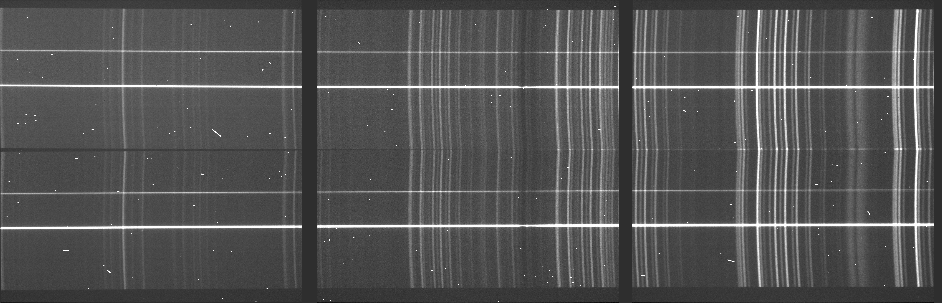
\includegraphics[width = 1.0\textwidth]{figures/3_pre_wav_cal.pdf}
    \caption{The science extension of a typical \textsc{polsalt} \gls{FITS} file after basic \gls{CCD} reductions have been completed.}
    \label{fig:polsalt_pre_wav_cal}
\end{figure}


\subsection{Splitting the POLSALT pre-calibration files}

The main struggle of formatting the files for \textsc{iraf} is that \textsc{iraf} does not handle the chosen \textsc{polsalt} \gls{FITS} file structures well, before or after the \textsc{polsalt} wavelength calibration. A typical \gls{FITS} file created by the \textsc{polsalt} basic \gls{CCD} reductions process has a primary header along with the various image extensions, all of which include both of the polarimetry beams. In an attempt to simplify the \textsc{iraf} reduction procedure it was decided to split the polarization beams into their own files, as the parameters of \textsc{iraf} tasks generally handle lists of files better than lists of cropping regions, and generally allowed for easier calibrations further down the \textsc{iraf} wavelength calibration process.
\prgph

The only steps added to splitting when preparing the \textsc{polsalt} data for \textsc{iraf} was the addition of the ability to crop and the creation of lists for easy automation when performing the wavelength calibrations. The cropping was decided on as \textsc{iraf} does not handle the empty rows and rows with overlapping traces well, specifically when it comes to the \textit{reidentify} task. Otherwise, whenever a design decision had to be made it was decided to stay as true to the \textsc{polsalt} pipeline decision as possible while still allowing \textsc{iraf} to handle the data.
\prgph

The \textsc{polsalt} files with basic \gls{CCD} reductions applied, namely files created by \textsc{polsalt} with a prefix of `mxgbp' (\S~\ref{subsec:polsalt}), are used as the starting point for the supplementary tool's splitting method. Running the split method finds all the \gls{FITS} files for wavelength calibration within the working directory, creates two empty \gls{HDU} structures for each sub-extension of the \gls{FITS} file, and appends all science and header data necessary for wavelength calibration to the relevant \gls{HDU} structure.

Many decisions are made when splitting the data, and it was decided to keep as true to the \textsc{polsalt} pipeline defaults as possible. Presets such as the row along which the data is split, and the amount of cropping applied to the data before appending, are defined but are freely controlled by the user. As this step creates multiple files, it was decided to keep the files for wavelength calibration as light as possible, with only the necessary science extension being copied over.

Fortunately, the \textsc{polsalt} \gls{FITS} files up to and including the basic \gls{CCD} reductions still has a conventional file structure with the only oddity being that the

\todo{Include O/E beam frame example}
\prgph

\todo{Mention steps before and how they return (especially) the file structure.
    All processes run in pipeline split with description of each and purpose. Focus on \textbf{why}.
    Header changes
}

\todo{Parsing polsalt mxgbp frame into something useable by IRAF and making sure the header reflects the changes}


\subsection{IRAF wavelength calibration}\label{subsec:IRAF_wav_cal}

\todo{All wavelength calibration steps - Again, focus on \textbf{why} instead of how
    \begin{itemize}
        \item Identify
        \item Reidentify
        \item Fitcoords
    \end{itemize}
}

\todo{(Optional) Transform (mention good for sanity checks which is not possible using the pure polsalt implementation)}


\subsection{Joining the wavelength calibrated files}

\todo{Return file structuring.}
There are means of accessing inner extensions via indexing within \textsc{iraf}, but this is unreliable for the various \textsc{iraf} tasks. As such, the extension structure needs to be handled such that \textsc{iraf} receives a flattened extension structure with proper extension headers.
\prgph

\todo{All processes run in pipeline join.
    Focus on \textbf{why}. Parsing \textsc{iraf} frames to be used by POLSALT and making sure the header and extensions reflect the changes}

\begin{figure}[t]
    \centering
    \includegraphics[width = 1.0\textwidth]{figures/3_post_wav_cal.pdf}
    \caption{The science extension of a \gls{FITS} file ready to be handed back to the \textsc{polsalt} pipeline.}
    \label{fig:polsalt_pre_wav_cal}
\end{figure}


\section{Additional Tools}\label{sec:add_tools}


\subsection{Cross correlation}

\todo{Why a cross correlation necessary and how it works}


\subsection{Skyline comparisons}

\todo{Again, why a skyline comparison necessary and how it works. Also, how the frame is transformed (\textsc{iraf} bypassed) and that the flux is not conserved so only for checking and not for science use.}


\section{General Reduction Procedure}\label{sec:red_proc}

\todo{General reduction procedure from raw data to finalized results
    \begin{itemize}
        \item This includes \textsc{polsalt} pre-reductions, splitting, \textsc{iraf} wavelength calibrations, checking, joining, and \textsc{polsalt} finalization. (Include Relative flux calibrations for `shape correcting' spectrum??)
    \end{itemize}
}
\chapter{Testing and Application}

This chapter contains an overview of the testing performed for the development of \stops\ (\autoref{sec:test_stops}) and the checking of the replaced wavelength solutions (\autoref{sec:test_wav}), as well as the application of \stops\ on observations (\autoref{sec:results_unpub}) and its application in publications (\autoref{sec:results_pub}).

% MARK: Test STOPS
\section[Testing \textsc{stops}]{Testing \stops} \label{sec:test_stops}

% No \polsalt\ tests or tests on pre-reduced \gls{FITS} files. (Trusted accurate)
% General discussion of testing (I.E. not this test was done specifically this source, more along the lines of these tests were done to check this issue, seen here using this source for example.)
The main challenge faced when developing \stops\ was ensuring that the software was compatible with both the \polsalt\ and \iraf\ file structures. As development is an iterative process, \stops\ was continually checked to ensure compatibility such that the varying \stops\ method inputs were correctly parsed, and that their outputs were parsable by the relevant \iraf\ tasks or \polsalt\ methods.

To this end, observations which were verified to have been accurately reduced were duplicated for testing purposes, allowing for continual checks of the \stops\ pipeline to be made during the development process. As the \stops\ \texttt{split} and \texttt{join} methods are designed to convert between the \polsalt\ and \iraf\ file structures, greater emphasis was made to ensure that the output of both methods provided accurate and consistent results.

% % Why the pipeline is better
% The rigorous error handling in \stops\ ensures that the user is informed of any issues that arise during the reduction process. This is particularly important as \stops\ was developed to enable a faster reduction process compared to that of pure \iraf\ or \polsalt.

% Reduction specific tests refer to tests performed to ensure no errant effects are introduced during the reduction process. These tests were designed to validate the accuracy and reliability of the \stops\ pipeline in producing scientifically accurate results.

% MARK: STOPS split tests
\subsection{Testing the \texttt{split} Method} \label{subsec:test_split}

The \stops\ \texttt{split} method requires any \polsalt\ pre-reduced (`mxgbp'- prefixed) \gls{FITS} files as input and outputs \iraf\ compatible (`(arc|beam)(O|E)'- prefixed) \gls{FITS} file structures. As no `split' \gls{FITS} files are created during pure \polsalt\ reductions, the \stops\ \texttt{split} method was tested by comparing the pre-reduced \polsalt\ files to the \texttt{split} method's output files, ensuring the correct structure and data integrity of the files handed off to \iraf.

\newcommand\mc[1]{\multicolumn{1}{c|}{#1}} % handy shortcut macro

\begin{table}[t]
    \centering
    \begin{tabular}{ccccccc}
        \hline
        Filename            & No. & Name    & Type       & Cards & Dimensions   & Format  \\ \hline
        \mc{\multirow{4}{*}{\parbox[c]{1.8cm}{mxgbpP\-20170328\-0054.fits}}}
                            & $0$ & \gls{PRIMARY} & PrimaryHDU & $161$   & ()           &  \\
        \mc{}               & $1$ & \gls{SCI}     & ImageHDU   & $19$    & ($3199$, $1028$) & float32 \\
        \mc{}               & $2$ & \gls{VAR}     & ImageHDU   & $8$     & ($3199$, $1028$) & float32 \\
        \mc{}               & $3$ & \gls{BPM}     & ImageHDU   & $8$     & ($3199$, $1028$) & uint8   \\
        \mc{beamo0054.fits} & $0$ & \gls{PRIMARY} & PrimaryHDU & $162$   & ($3199$, $474$)  & float32 \\
        \mc{beame0054.fits} & $0$ & \gls{PRIMARY} & PrimaryHDU & $162$   & ($3199$, $474$)  & float32 \\ \hline
    \end{tabular}
    \caption{A comparison of the \polsalt\ pre-reduced \texttt{mxgbpP201703280054.fits} file, and the \stops\ \texttt{split} \texttt{beamo0054.fits} and \texttt{beame0054.fits} file contents.}
    \label{table:split_info}
\end{table}


\autoref{table:split_info} shows the \gls{FITS} file information for the files before and after splitting. The split \gls{FITS} files contain the split \gls{SCI} extension data and the \gls{PRIMARY} header from the pre-reduced files, with any Header or Data differences mentioned below.

The header is left mostly untouched, and is only updated to represent the new data type and shape:
the `BITPIX' value is updated, from $8$ to $-32$, and the `NAXIS' value is updated, from $0$ to $2$;
the `NAXIS1' and `NAXIS2' keywords are added, and their values are set to the new split \gls{SCI} data shape;
and the `EXTEND' keyword is removed.%
\footnote{The `EXTEND' keyword indicates that the \gls{FITS} file contains multiple extensions while the `NAXIS1' and `NAXIS2' keywords indicate the shape and size of the data stored in the relevant extension.}
This accounts for the discrepancy in the `Cards' between the \polsalt\ and \stops\ file header entries in \autoref{table:split_info}.

\begin{figure}
    \centering
    \begin{subfigure}[b]{\textwidth}
        \centering
        \includegraphics[width=\textwidth]{4_diff_O.pdf}
        \caption{The difference in the \gls{SCI} extensions, for the `O' polarization beam.}
        \label{subfig:diff_split_O}
    \end{subfigure}
    \hfill
    \begin{subfigure}[b]{\textwidth}
        \centering
        \includegraphics[width=\textwidth]{4_diff_E.pdf}
        \caption{The difference in the \gls{SCI} extensions, for the `E' polarization beam.}
        \label{subfig:diff_split_E}
    \end{subfigure}
    \caption{The difference between the \polsalt\ pre-reduced (`mxgbp'- prefixed) \gls{FITS} files and the \stops\ `split' (`(arc|beam)(O|E)'- prefixed) files. Figures created using both the \polsalt\ \texttt{Raw image reduction} and \stops\ \texttt{split} method outputs.}
    \label{fig:split_diff}
\end{figure}

\autoref{fig:split_diff} shows that the \polsalt\ \gls{SCI} data is unmodified when copying the data to the \stops\ \gls{FITS} file, but only includes half of the data, for the relevant $O$- or $E$-polarization beam, \autoref{subfig:diff_split_O} and \autoref{subfig:diff_split_E}, respectively, with a cropping which defaults to $40$~pixels (see \autoref{subsec:stops_split}), introduced to the top- and bottom-most rows of the \polsalt\ data. This accounts for the discrepancy in the `Dimensions' between the \polsalt\ and \stops\ files in \autoref{table:split_info}.

This output file structure was chosen for \iraf\ compatibility, and was tested for robustness over multiple grating and articulation angles, as well as with various data sets to ensure that the \texttt{split} method was robust and reliable.

% MARK: STOPS join tests
\subsection{Testing the \texttt{join} Method} \label{subsec:test_join}

The \texttt{join} method requires both an \iraf\ database with wavelength solutions (or a custom wavelength solution) for both polarimetric beams and the \polsalt\ pre-reduced files as input and outputs \polsalt\ \texttt{spectra extraction} compatible (`wmxgbp'- prefixed) \gls{FITS} file structures. Ensuring that the output format was correct was paramount as the \polsalt\ \texttt{spectra extraction} method is unable to process the files otherwise, thus halting the reduction process. Thankfully, the \texttt{join} method output could be compared to the \polsalt\ \texttt{wavelength calibration} method output files, ensuring that any changes introduced by the \stops\ pipeline were well characterized.

\newcommand\mc[1]{\multicolumn{1}{c|}{#1}} % handy shortcut macro

\begin{table}[t]
    \centering
    \begin{tabular}{}
        \hline
        \\ \hline
        \hline
    \end{tabular}
    \caption{}
    \label{table:join_info}
\end{table}


\autoref{table:join_info} shows the \gls{FITS} file information for both the \polsalt\ and \stops\ wavelength calibrated files. Other than the `Dimensions' of each `ImageHDU' extension,%
\footnote{The `Dimensions' differ due to the before mentioned cropping of the top- and bottom-most rows of the data.}
the \gls{FITS} files are identical in structure.

Although the `Cards' count is the same, minor differences across the headers are present. The `HISTORY' keyword, which contains the \polsalt\ `CRCLEAN' parameters and which default to `upper= 4.0, lower= 1.5, sigmaveto= 2.0', is left as `None' in the \stops\ file.%
\footnote{The \polsalt\ pipeline performs cosmic ray cleaning using a $10\sigma$ spike to cull cosmic rays. See the \polsalt\ \protect\href{https://github.com/saltastro/polsalt/blob/master/polsalt/specpolwavmap.py\#L132}{source code} for more information.}
Although \stops\ performs cosmic ray cleaning (see \autoref{subsec:stops_join}), the parameters are not stored in the header as \polsalt\ and \stops\ implement different methods for cosmic ray cleaning. Other minor differences such as the date-times stored in the `SAL-TLM' and `SMOSAIC' keywords may also differ as they contain the date-times relating to the completion of the \polsalt\ pre-reductions. This accounts for the differences in the `Cards' between the \polsalt\ and \stops\ file header entries in \autoref{table:join_info}.

\begin{figure}
    \centering
    \begin{subfigure}[b]{\textwidth}
        \centering
        \includegraphics[width=\textwidth]{4_diff_SCI.pdf}
        \caption{The difference in the \gls{SCI} extensions.}
        \label{subfig:join_SCI}
    \end{subfigure}
    \hfill
    \begin{subfigure}[b]{\textwidth}
        \centering
        \includegraphics[width=\textwidth]{4_diff_VAR.pdf}
        \caption{The difference in the \gls{VAR} extensions.}
        \label{subfig:join_VAR}
    \end{subfigure}
    \hfill
    \begin{subfigure}[b]{\textwidth}
        \centering
        \includegraphics[width=\textwidth]{4_diff_BPM.pdf}
        \caption{The difference in the \gls{BPM} extensions.}
        \label{subfig:join_BPM}
    \end{subfigure}
    \hfill
    \begin{subfigure}[b]{\textwidth}
        \centering
        \includegraphics[width=\textwidth]{4_diff_WAV.pdf}
        \caption{The difference in the \gls{WAV} extensions.}
        \label{subfig:join_WAV}
    \end{subfigure}
    \caption{The difference of the \gls{FITS} file extensions between the \polsalt\ and \stops\ (`wmxgbp'- prefixed) wavelength calibrated files. Figures created using both the \polsalt\ and \stops versions of the \polsalt\ \texttt{spectral extraction} input.}
    \label{fig:join_in_out_diff}
\end{figure}

\autoref{fig:join_in_out_diff} shows the differences in the data between the \polsalt\ and \stops\ wavelength calibrated files. It can be seen that the \gls{VAR} extensions (\autoref{subfig:join_VAR}) are identical. The \gls{SCI} extensions (\autoref{subfig:join_SCI}) differ only in that the cosmic ray cleaning has been applied to the \stops\ data, whereas the \polsalt\ data applies a mask to the cosmic rays using the \gls{BPM} extension (\autoref{subfig:join_BPM}). The \gls{BPM} and \gls{WAV} extensions (\autoref{subfig:join_WAV}) are also masked to account for the valid wavelength calibrated region. The \gls{WAV} extensions contain the differing wavelength solutions and as such naturally differ. This accounts for the differences in the data between the \polsalt\ and \stops\ files.

Finally, the \stops\ \texttt{join} method was tested to ensure compatibility and correctness of the output data in comparison to \polsalt. This involved testing the \texttt{join} method with various data sets to ensure that the output files were accurate and consistent.

% MARK: Check Wav. Cal.'s
\section{Wavelength Solution Checks} \label{sec:test_wav}

% No \iraf\ tests or tests on \iraf\ \gls{FITS} files. (Trusted accurate)
The secondary challenge encountered when developing \stops\ was ensuring that the wavelength solutions parsed by \stops\ were unaffected by the pipeline and that they were consistent with those created by \polsalt. This was achieved through the \texttt{correlate} and \texttt{skylines} methods, which were designed to validate the wavelength solutions produced by \iraf.

Before the \polsalt\ wavelength calibrations were replaced with the \iraf\ wavelength calibrations, the accuracy of the new wavelength solutions needed to be validated. This was done both through the \iraf\ tasks, ensuring an accurate wavelength solution, and through the \stops\ \texttt{correlate} and \texttt{skylines} methods, allowing the integration of the wavelength solutions to be validated.
% \gls{RMS} results returned from each

% Wavelength solution validation from correlate and skylines results.
%     \begin{itemize}
%         \item RMS comparisons between \polsalt\ and \iraf\ to quantify differences.
%         \item Any Figures for RMS comparisons or wavelength validation?
%     \end{itemize}

% Testing \iraf\ wavelength solution
% \begin{itemize}
%     \item The \texttt{skylines} and \texttt{correlate} outputs are tests of the wavelength calibration.
% \end{itemize}

% Wavelength solution tests were conducted to validate the accuracy of the \stops\ wavelength calibration process. This included:
% \begin{itemize}
%     \item Full frame wavelength solution checks to ensure comprehensive calibration.
%     \item O/E correlation checks to verify the consistency of the wavelength solutions.
%     \item RMS comparisons between \polsalt\ and \stops\ to quantify differences.
% \end{itemize}

% \todo{Insert table comparing RMS values of wavelength solutions from \polsalt\ and \stops.}

% \todo{Insert figure showing full frame wavelength solution plots.}

% The \texttt{correlate} and \texttt{skylines} methods were tested for accuracy and performance. Key aspects of the testing included:
% \begin{itemize}
%     \item Verifying the accuracy of the cross-correlation function against known standards.
%     \item Ensuring skyline identification was accurate and consistent.
%     \item Performance testing with large data sets to ensure efficiency.
% \end{itemize}

% \todo{Insert graph showing correlation results with known standards.}

% MARK: WAV Corr. Checks
\subsection{Cross Correlation Checks} \label{subsec:test_corr}

The \texttt{correlate} method returns plots validating the wavelength solutions and so only has to accept the \polsalt\ \texttt{spectra extraction} (`ecwmxgbp'- prefixed) method output files as input.

% \begin{itemize}
%     \item Testing correlate functionality using `offset', comparisons of arcs, FSRQ's and BLLac's.
%     \item Any figures showing correlation tests?
% \end{itemize}

% \todo{Insert figure illustrating cross correlation accuracy.}

% MARK: WAV Sky. Checks
\subsection{Sky Line Checks} \label{subsec:test_sky}

The \texttt{skylines} method returns plots validating the wavelength solutions and so only has to accept either the \iraf\ \texttt{transform} task or \stops\ \texttt{join} method output files as input.

% \begin{itemize}
%     \item Testing skylines using known spectral sky lines.
%     \item Any figures showing skyline tests?
% \end{itemize}

% \todo{Insert figure illustrating skyline identification accuracy.}

% MARK: Results Unpub.
\section[Application of \textsc{stops}]{Application of \stops} \label{sec:results_unpub}

% MARK: Science Targets
\subsection{Spectropolarimetric Science Targets}

% Tested using 3C 279, 4C+01.02, and preliminary testing data provided by David. \todo{VERIFY CORRECT}

\subsubsection{Background Information}

% Background information on each object.
% \todo{Tabulate sources used, with their properties.}

\subsubsection{Reduction Steps}

% Detailed reductions steps performed on each object.

\subsubsection{Results and Comparison}

% Comparison of \polsalt\ results to those obtained using the \stops\ pipeline.
% \todo{Insert figures showing comparison plots of polarization parameters from \polsalt\ and \stops.}

% MARK: Spec.pol. Standards
\subsection{Spectropolarimetric Standards}

% Testing included the use of spectropolarimetric standards, comprising four highly polarized and two non-polarized objects. \todo{VERIFY CORRECT}

\subsubsection{Background Information}

% Background information on each object. / General discussion of sources used as part of testing
% \todo{Insert table listing the spectropolarimetric standards used, with their properties.}

% The sources used for testing included a range of spectropolarimetric standards, both highly polarized and non-polarized objects. The tests aimed to check for issues such as data integrity, consistency of wavelength calibration, and accuracy of polarization measurements.

\subsubsection{Reduction Steps}

% Detailed reductions steps performed on each object. Highlight any differences in reduction steps compared to science targets.

\subsubsection{Results and Comparison}

% Comparison of \polsalt\ results to those obtained using the \stops\ pipeline.
% Science results, what the results can tell us and why it is useful,
% also comparison of results to FORS1/2 published data, focus on the polarization results.

% \todo{Insert figures showing comparison plots of polarization parameters from \polsalt\ and \stops.}

% MARK: Results Pub.
\section{Application in Publications} \label{sec:results_pub}

% \subsection{} for each publication
% Summarize the results of the publications appended to appendix.


% \begin{itemize}
%     \item Hester paper(s)
%     \item Joleen proceedings and work
%     \item My proceedings
% \end{itemize}

\chapter{Conclusions} \label{ch:05}

% • Background and motivation
% - What are you talking about?
% - What questions are you trying to answer?
% - What’s the bigger picture?
% • What did you do?
% - What did you observe?
% - Experimental and analysis method(s)
% - What theory/models are you using?
% • What did you find?
% • What does it mean? What do you conclude?

\todo{A summary of the dissertation, main focus on the results and that the supplementary pipeline is a success since it allows an alternate method using IRAF to wavelength calibrate the polsalt data.}

\section{Future Work}

% Summarize state of Astronomical software - IRAF & POLSALT
It is possible to complete the data reductions of \gls{SALT}/\gls{RSS} spectropolarimetric data using only the \polsalt\ pipeline.
This does not negate the fact that better tools and software better allow us to focus on the results of observations rather than the data reduction process.
Due to the limitations inherent in software designed for use strictly as a pipeline, there is a lack of flexibility in data reduction processes, an over-reliance on the software to provide accurate results, and a lack of urgency when keeping `completed' software up-to-date.
% Point in case, \polsalt\ is written in Python~$2$, which was deprecated in $2020$, while \iraf\ is referred to as legacy software, receiving only community driven support.

% New software - Python trend
Newer software, such as Python~$3$, is trending for data reductions due to the compatibility and maintenance with modern systems, the rich packages available for use, and an active development environment.
In this regard, the development of the \stops\ software is a step in the right direction, providing a channel for alternate wavelength calibrations to be integrated with \polsalt, while still maintaining the integrity of the data reduction process.
That said, the software is not without its limitations.

% STOPS
% Future use guaranteed in data reductions
% Limited by \polsalt\ development
Future work would involve the continued development and maintenance of the \stops\ software, further integration of the software with \polsalt, and possibly the development of a user-friendly interface or modification of the \polsalt\ \gls{GUI} to include the \stops\ functionality.

Wavelength calibrations completed in Python~$3$, with the help of \gls{PyPI} packages, are already supported, but further integration of non-standard wavelength solutions would also be beneficial, as the current wavelength solutions are limited to Chebyshev and Legendre polynomials.
% What will be discussed, however, is the structure of the wavelength solutions created through Python to be later reintroduced to the \polsalt\ pipeline. The solutions must be stored such that the `$x$' and `$y$' orders of the solution, as well as all the coefficients ($C_{00}$ to $C_{xy}$) making up the solution, separated by new lines, are included. The only limitations to the names of the solution files is that they must make mention of the specific $O$- or $E$-beam as well as the wavelength solution type (e.g. `Chebyshev', `Legendre', etc.).


% MARK: Appendix
% New chapter count type
\appendix
% Roman numerals for Appendix numbering
% \renewcommand{\thechapter}{\Roman{chapter}}
\Chapter{Commands for the Reduction Process}{A minimum working example}

\todo{Add minimum working example of reduction process here.}

% MARK: Appendix - source code
% https://www.overleaf.com/learn/latex/Code_listing
\chapter[\textsc{stops} Source Code]{\stops\ Source Code} \label{app:code}

This section of Appendix includes all the major \stops\ source code files related to the reduction process. Files such as those related to python initialization, testing directories, and other non-essential modules have been excluded for brevity and clarity.

% MARK: __main__ source
\lstinputlisting[
    language=python,
    style=STOPS,
    caption={The source code for \textbf{\_\_main\_\_.py}},
    label=source:main]
{__main__.py}
\clearpage

% MARK: split source
\lstinputlisting[
    language=python,
    style=STOPS,
    caption={The source code for \textbf{split.py}},
    label=source:split]
{split.py}
\clearpage

% MARK: join source
\lstinputlisting[
    language=python,
    style=STOPS,
    caption={The source code for \textbf{join.py}},
    label=source:join]
{join.py}
\clearpage

% MARK: cross_correlate source
\lstinputlisting[
    language=python,
    style=STOPS,
    caption={The source code for \textbf{cross\_correlate.py}},
    label=source:cross]
{cross_correlate.py}
\clearpage

% MARK: skylines source
\lstinputlisting[
    language=python,
    style=STOPS,
    caption={The source code for \textbf{skylines.py}},
    label=source:sky]
{skylines.py}

% Possible Macro for code listings
% https://en.wikibooks.org/wiki/LaTeX/Source_Code_Listings


% MARK: Back matter
% No chapter count type
\backmatter
\bibliographystyle{plainnat}
\bibliography{references}

% \printglossaries
% Longest abbreviation so the column width can be set
% \glssetwidest{\gls{STOPS}}
\printglossary[type=main, title={Glossary}]

\end{document}
